\documentclass{article}
\usepackage[utf8]{inputenc}
\usepackage{graphicx}
\graphicspath{{Imagens/}}


\title{ Principal Components Analists \\ Algebra Linear}
\date{06/12/2022}
\author{Augusto Rodrigo Camblor Santos\\Gabriela Duarte Maciel\\}
\usepackage{geometry}
\geometry{a2paper,left=2cm,right=10mm,top=1cm,bottom=3cm}

\begin{document}


\maketitle


\begin{itemize}
\item Dataset selecionado. \\ \\
import pandas as pd\\
import numpy as np\\
import matplotlib.pyplot as plt\\
import random as rd\\
from sklearn import preprocessing \\
from sklearn.decomposition import PCA\\ \\
data = pd.read\textunderscore csv("./input/ProjetosRenunciaFiscal1.csv", encoding="utf-8") \\ \\
dataTitulo = data["TITULO\textunderscore PROJETO"]\\ \\
del data["TITULO\textunderscore PROJETO"]\\
del data["CNPJ\textunderscore PROPONENTE"]\\
del data["Unnamed: 0"]\\
del data["Unnamed: 2"]\\
del data["UF\textunderscore PROPONENTE"]\\
del data["SITUACAO\textunderscore REGISTRO"]\\
del data["RAZAO\textunderscore SOCIAL\textunderscore PROPONENTE"]\\ \\
data["LEI\textunderscore 8313"]= data["LEI\textunderscore 8313"].str.replace(",", ".")\\
data["ART1"] = data["ART1"].str.replace(",", ".")\\
data["ART1A"]= data["ART1A"].str.replace(",", ".")\\
data["ART3"] = data["ART3"].str.replace(",", ".")\\
data["ART3A"]= data["ART3A"].str.replace(",", ".")\\
data["ART39"]= data["ART39"].str.replace(",", ".")\\
data["FUNCINES"] = data["FUNCINES"].str.replace(",", ".")\\
data["TOTAL\textunderscore CAPTADO"]= data["TOTAL\textunderscore CAPTADO"].str.replace(",", ".")\\ \\
print(data)\\
print(data.head())\\
print(data.shape)\\ \\
\end{itemize}

\begin{itemize}
\item Cálculo da matriz de covariância, autovalores e autovetores.\\ \\
scaled\textunderscore data = preprocessing.scale(data)\\ \\
dataIndex = object\\ \\
for gene in data.index:\\
    dataTitulo = data.loc[gene] \\ \\
pca = PCA()\\
pca.fit(scaled\textunderscore data)\\
pca\textunderscore data = pca.transform(scaled\textunderscore data)\\ \\
per\textunderscore var = np.round(pca.explained\textunderscore variance\textunderscore ratio\textunderscore  * 100, decimals = 1)\\
labels = ['PC' + str (x) for x in range (1, len(per\textunderscore var)+1)]\\ \\
plt.bar(x=range(0, len(per\textunderscore var)), height=per\textunderscore var, tick\textunderscore label = labels)\\
plt.ylabel('Percentage of Explained Variance')\\
plt.xlabel('Principal Component')\\
plt.title('Scree Plot')\\
plt.show()\\ \\
\end{itemize}

\begin{itemize}
\item Dois maiores autovalores.\\ \\
pca\textunderscore df = pd.DataFrame(pca\textunderscore data, index = data, columns = labels)\\ \\
plt.scatter(pca\textunderscoredf.PC1, pca\textunderscore df.PC2)\\
plt.title('My PCA Graph')\\
plt.xlabel('PC1'.format(per\textunderscore var))\\
plt.ylabel('PC2'.format(per\textunderscore var))\\ \\
plt.show()\\ \\
\end{itemize}

\begin{itemize}
\item Plotagem das colunas correspondentes aos dois autovalores.\\ \\
loading\textunderscore scores = pd.Series(pca.components\textunderscore[0], index = dataTitulo)\\
sorted\textunderscore loading\textunderscore scores = loading\textunderscore scores.abs().sort\textunderscore values(ascending=False)\\
top\textunderscore 10\textunderscore projetos = sorted\textunderscore loading\textunderscore scores[0:10].index.values\\
print(loading\textunderscore scores[top\textunderscore 10\textunderscore projetos])\\ \\
\end{itemize} 
\begin{itemize}
    \item Link do repositório do GitHub
    \newline(Link:
    Link do repositório no GitHub: https://github.com/AugustoRC/P2Algebra
);
\end{itemize}\\ \\

\begin{itemize}

\item Prints dos resultados gerados:
\end{itemize}

\begin{figure}[!h]
\centering
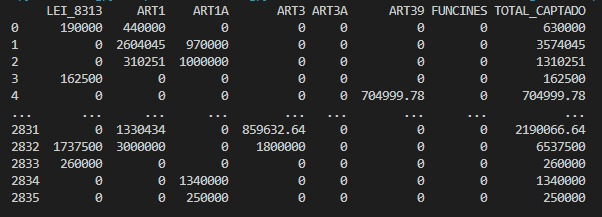
\includegraphics[width=10cm]{banco de dados int.jpg}
\caption{Banco de dados selecionado.}
\label{fig:banco de dados int.jpg}
\end{figure}

\begin{figure}[!h]
\centering
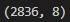
\includegraphics[width=10cm]{banco de dados tratado.jpg}
\caption{Banco de dados após o tratamento.}
\label{fig:banco de dados tratado.jpg}
\end{figure}

\begin{figure}[!h]
\centering
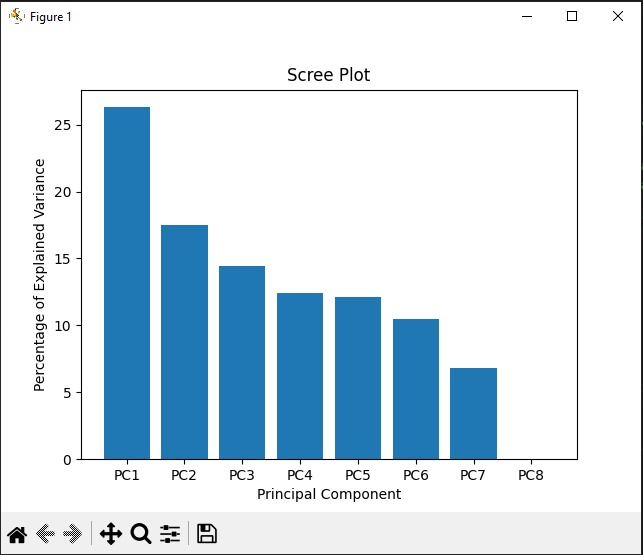
\includegraphics[width=10cm]{pci.jpg}
\caption{Cálculo de autovetores e autovalores.}
\label{fig:pca.jpg}
\end{figure}

\begin{figure}[!h]
\centering
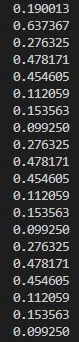
\includegraphics[width=10cm]{autovalores.jpg}
\caption{Maiores Autovalores.}
\label{fig:autovalores.jpg}
\end{figure}

\begin{figure}[!h]
\centering
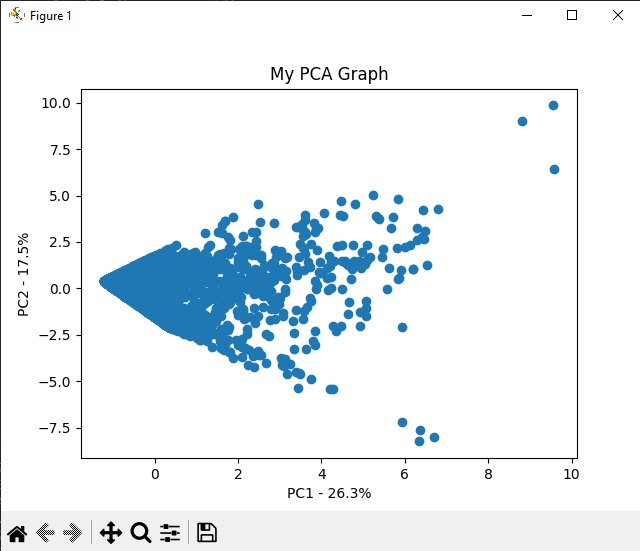
\includegraphics[width=10cm]{coordenadas.jpg}
\caption{Plotagem dos maiores autovalores.}
\label{fig:coordenadas.jpg}
\end{figure}\\



\end{document}